\documentclass[onecolumn]{article}
\usepackage{graphicx}
\usepackage{float}
\usepackage{hyperref}
\restylefloat{figure}
\begin{document}

\title{Boundary-initial value problems with the advection-diffusion equation}
\author{Arjen Markus}

\maketitle

\section*{Introduction}
While the advection-diffusion equation is, mathematically and physically
speaking a fairly simple one, especially in one dimension, finding analytical
solutions for various concrete problems is challenging.

To be precise, the partial differential equation we consider here in various forms is:
\begin{eqnarray}
\label{advdiff}
    \frac{\partial C}{\partial t} + u \frac{\partial C}{\partial x} &=& D \frac{\partial^2 C}{\partial x^2} + k C
\end{eqnarray}

\noindent where $C$ is the concentration of some substance or the temperature or some other scalar quantity,
$u$ the flow velocity and $D$ the diffusion coefficient. The last term is a reaction term, most likely a
reaction quantifying the rate of decay, such as with a radiative substance.

We will consider a variety of boundary and initial conditions and try to find an analytical solution, mostly
by means of the Laplace transformation.

\section*{Point mass spreading out}
\label{pointmass}
A classical problem is where there is a point source at the origin representing a finite mass, which then
spreads out into infinity in a stagnant medium, so that the flow velocity is zero. The initial condition
can be written as:
\begin{eqnarray}
\nonumber    C &=& M \delta(x)
\end{eqnarray}
\nonumber (with a slightly problematic interpretation of the physical units -- $C$ as the concentration and $M$ as the total mass).

To solve equation \ref{advdiff} with in this case $u = 0$ and $k = 0$ we use the Laplace transformation. The Dirac $\delta$
function is always a tricky thing to handle, but we can interpret the initial condition in the following way: at
time $t = 0$ there is a mass $M$ present which then spreads out. So, if we integrate the solution over the entire
domain, the result must be that same mass. If we apply the Laplace transformation to a part of the x-axis just off of
the origin, then the initial condition is simply $C = 0$ for $x > 0$, similarly for $x < 0$. Then the transformed equation becomes:
\begin{eqnarray}
\nonumber    s \Gamma &=& D \frac{d^2 \Gamma}{d x^2} ~~~~~~~x > 0
\end{eqnarray}
\noindent with the straightforward solution:
\begin{eqnarray}
\nonumber    \Gamma &=& A e^{-x \sqrt{s/D}} + B e^{+ \sqrt{s/D}}
\end{eqnarray}

The boundary conditions to determine $A$ and $B$ are:
\begin{itemize}
\item
The solution remains finite.
\item
The total mass is constant and equal to $M$.
\end{itemize}

The first condition leads to: $A = 0$ for $x < 0$ and $B = 0$ for $x > 0$. Since the concentration $\Gamma$ must be
continuous, $A_{x>0} \equiv B_{x<0}$. And the second condition leads to:
\begin{eqnarray}
\nonumber   \int^{\infty}_{-\infty} C(x,t) dx &=& M  ~~~ t \geq 0
\end{eqnarray}

Taking the Laplace transform, as we want to turn this into a condition on $\Gamma$:\footnote{At first, when I wrote
this down, I assumed I could simply replace $C$ by $\Gamma$, but that leads to the \emph{wrong} solution. The condition
says something about the time domain, hence the Laplace transformation is required.}

\begin{eqnarray}
\nonumber   L( \int^{\infty}_{-\infty} C  dx ) &=& L(M) \\
\nonumber   \int^{\infty}_{-\infty} \Gamma dx &=& \int^{0}_{-\infty} A e^{x \sqrt{s/D}} dx + \int^{\infty}_{0} A e^{-x \sqrt{s/D}} dx \\
\nonumber                                     &=& 2A / \sqrt{s/D} \\
\nonumber                                     &=& M/s
\end{eqnarray}

We therefore need to find the inverse of $\frac{1}{2} M e^{-x \sqrt{s/D}} / \sqrt{sD}$ to get the analytical solution.

The solution is:\footnote{The WolframAlpha site is very useful for this sort of calculations -- \url{www.wolframalpha.com/input?i=inverse+Laplace+transform}.}
\begin{eqnarray}
\nonumber   C(x,t) &=& \frac{M}{2 \sqrt{\pi D t}} e^{-x^2/4Dt}
\end{eqnarray}

So, the maximum concentration diminishes as $1/\sqrt{t}$ and the width (defined as the distance from the origin where
the concentration is half that of the maximum) increases as $\sqrt{t}$.

\subsection*{Steady flows and decay processes}
With a steady flow to the right ($u \neq 0$) and the same boundary/initial conditions, we can simply replace $x$ by $x-ut$
to get a moving "cloud". The substitution causes the term $u \partial C / \partial x$ to disappear and leave all other
terms intact.

With a decay process ($k = -r < 0$) we can solve the equation by introducing a factor $e^{-rt}$.

The solution for a situation of a point source of a decaying substance (a radio-active isotope, say) in a moving medium
is then:
\begin{eqnarray}
\nonumber   C(x,t) &=& \frac{M}{2 \sqrt{\pi D t}} e^{-(x - ut)^2/4Dt} ~e^{-rt}
\end{eqnarray}

The reason we can simply introduce the decay factor like this is that all of the substance has the same "age" -- it
is introduced at time $t = 0$ into the system and after that nothing new is introduced.

If the point mass is replaced by a continuous source at the origin, then things are very different. The solution
to that problem is no longer obtained by a simple translation, as the position of the substance changes with respect
to the source or by a simple decay factor, as new mass is continuously introduced and therefore the decay does
not have the same overall effect on all the substance. We need to look for another solution.

% https://nickelnine37.github.io/the-diffusion-equation.html

\section*{Continuous point source}
If we have a continuous constant point source at the origin (and no decay), then this can be interpreted as a change in the second condition
we introduced in the previous section. Instead of the total mass being constant, we get:
\begin{eqnarray}
\nonumber   \int^{\infty}_{-\infty} C(x,t) dx &=& Lt  ~~~ t \geq 0
\end{eqnarray}

\noindent where $L$ is the mass flux per unit of time, leading to a term $L/s^2$ instead of $M/s$.

With a similar analysis as before, we now get the Laplace transform:
\begin{eqnarray}
   \Gamma &=& \frac{L} {2 s \sqrt{sD} } e^{-x \sqrt{s/D}}
\end{eqnarray}

The concentration $C(x,t)$ can be expressed in elementary functions as:
\begin{eqnarray}
   C(x,t) &=& 2L \sqrt{\frac{t}{\pi D}} e^{-x^2/4Dt} H_{-2}\Bigl(\frac{x}{\sqrt{2Dt}}\Bigr)
\end{eqnarray}

\noindent where $H_{-2}$ is an Hermite "polynomial":\footnote{As the Wolfram Mathworld site did not explain this function, I looked
it up via Google and found \url{https://math.stackexchange.com/questions/2238662/do-hermite-polynomials-exist-for-negative-integers}.}
\begin{eqnarray}
     H_{-2}(x) &=& \frac{1}{2} \Bigl(1 - \sqrt{\pi} e^{x^2} erfc(x) \Bigr)
\end{eqnarray}

\section*{Water entering a tube}
As the expressions are becoming unwieldy, let us focus on a different problem: a half-infinite "tube" with a steady flow
and a decaying substance. The substance enters the tube at a given concentration $C = 1$. The boundary conditions
are now:
\begin{itemize}
\item
The concentration at $x = 0$ is 1.
\item
The concentration remains finite for $x \rightarrow \infty$.
\end{itemize}
For simplicity we take the initial condition to be: $C = 0$ at $t = 0$.

The boundary condition for the Laplace transform is, of course: $\Gamma(0,s) = 1/s$.

Equation \ref{advdiff} becomes, after the transformation:
\begin{eqnarray}
     s \Gamma + u \frac{d \Gamma}{dx} &=& D \frac{d^2 \Gamma}{dx^2}
\end{eqnarray}

The solution is of the form:
\begin{eqnarray}
\nonumber    \Gamma        &=& A e^{\lambda_- x} + B e^{\lambda_+ x} \\
\nonumber    \lambda_{\pm} &=& \frac{u}{2D} \pm \sqrt{\frac{u^2}{4D^2} + \frac{s}{D}}
\end{eqnarray}

For the concentration to remain finite as $x \rightarrow \infty$ we need to choose $B = 0$.

For the concentration to be 1 at $x = 0$, coefficient $A$ for the transform must be $1/s$. Therefore the transformed
solution is:
\begin{eqnarray}
\nonumber    \Gamma        &=& e^{x \bigl( \frac{u}{2D} - \sqrt{\frac{u^2}{4D^2} + \frac{s}{D}} \bigr)} / s
\end{eqnarray}

Unfortunately, the Wolfram Alpha website does not provide an answer. It does provide one, if we leave out the factor $1/s$:
\begin{eqnarray}
\nonumber     C^*(x,t)     &=& \frac{x}{\sqrt{4 \pi D t^3}} e^{ux/2D -u^2t/4D - x^2 /4Dt}
\end{eqnarray}

We can, however, find a solution, be it not in closed form, by integrating $C^*$ over time, as this is equivalent to
multiplying the Laplace transform by a factor $1/s$:\footnote{See for instance \url{https://en.wikipedia.org/wiki/Laplace_transform\#Properties_and_theorems}.}
\begin{eqnarray}
\nonumber     C(x,t)     &=& \int_0^t \frac{x}{\sqrt{4 \pi D \tau^3}} e^{ ux/2D -u^2 \tau/4D - x^2 /4D \tau} d \tau
\end{eqnarray}

There is, however, something wrong with this solution, as can easily be seen from the graphs in Figure \ref{waterTube}:
\begin{figure}[H]
\caption{Solution for several values of the time t, as function of x}
\label{waterTube}
\begin{center}
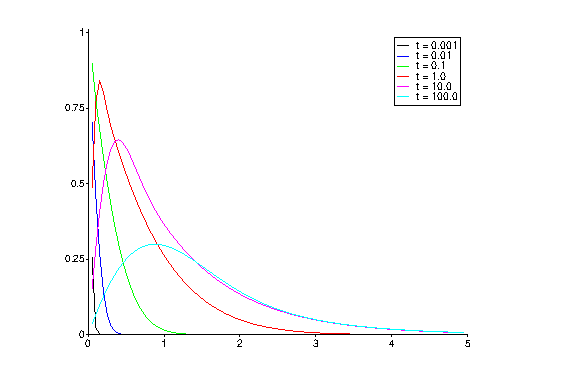
\includegraphics[width=0.9\textwidth]{water_tube.pdf}
\end{center}
\end{figure}

The transformed solution shows that the concentration should be constantly 1 at $x = 0$ (since the function reduces to $\Gamma(s) = 1/s$). But the numerical integration shows
a maximum that moves with time and the solution at $x = 0$ is not 1. The reason for this is unclear, I can only conclude that I
have made a mistake somewhere. It very much looks like the solution is for a point mass that spreads out under the influence
of flow and diffusion, rather than a continuous inflow via the left boundary.


\section*{A related problem -- uniform source}
In the so-called \emph{Constituent-oriented age and residence time theory} (or CART) \cite{ConceptOfAgeMarineModelling}, equations
like the advection-diffusion equations play a role but with a source term that is not concentrated in space.
The basic one-dimensional equations for water entering a channel (or a tube) as before, but now \emph{replacing} the water
that is already there are (ignoring diffusion):
\begin{eqnarray}
\nonumber    \frac{\partial C}{\partial t} + u \frac{\partial C}{\partial x} &=& 0 \\
\nonumber    \frac{\partial A}{\partial t} + u \frac{\partial A}{\partial x} &=& C
\end{eqnarray}

In these equations the variable $C$ is the concentration of a tracer and the variable $A$ is the so-called
age concentration. The \emph{age} $a$ of the water (or the tracer) is then calculated as $a = A/C$.

The situation we are going to examine is this:
\begin{itemize}
\item
The water in the channel is being replaced by water coming in on the left-hand side at $x = 0$.
\item
This water gradually replaces the water that is already there.
\item
With the boundary and initial conditions, $C = 1$ at $x = 0, t \geq 0$ and $C = 1$ at $t = 0, x \geq 0$, the
concentration of $C$ remains 1.
\item
The equation for the age concentration $A$ therefore reduces to:
\begin{eqnarray}
    \frac{\partial C}{\partial t} + u \frac{\partial C}{\partial x} ~=~ 1
\end{eqnarray}
\item
The water that is present in the channel at $t = 0$ will age as time proceeds and since all the water
is there from the start, the water age is uniform over the undisturbed part of the channel, increasing
with the same rate as time itself.
\item
This water is being replaced, however, by water entering the channel via the left-hand side, which has
an age $a = 0$, or, equivalently, an age concentration $A = 0$. As it travels along the channel, replacing
more an more original water, it will age as well.
\end{itemize}

\emph{Note:}
The CART theory aims to determine the age and residence times of a tracer in a water system and the above equation
arises in a slightly more complicated form. Here we have dropped the dispersion term for simplicity (much
more can be said about that, but that would boil down to discussing the theory as such and that does not
fit the scope).

The boundary and initial conditions for the above problem are:
\begin{eqnarray}
     C &=& 0 ~~~~~~ (x = 0) \\
     C &=& 0 ~~~~~~ (t = 0) \\
     C &<& \infty ~~~~~~(x \rightarrow \infty)
\end{eqnarray}

Using the Laplace transformation we get the equation:
\begin{eqnarray}
    s \Gamma + u \frac{d \Gamma}{d x} &=& \frac{1}{s}
\end{eqnarray}

\noindent which is straightforward to solve, resulting in:
\begin{eqnarray}
    \Gamma &=& \frac{1}{s^2} \Bigl ( 1 - e^{-xs/u} \Bigr )
\end{eqnarray}

The inverse transform gives:
\begin{eqnarray}
    C(x,t) &=& (x/u - t) H(t - x/u) + t
\end{eqnarray}
\noindent $H(y)$ is the Heaviside step function:
\begin{eqnarray}
    H(y) &=& 0 ~~~~~~ (y < 0) \\
         &=& 1 ~~~~~~ (y \geq 0)
\end{eqnarray}

To interpret this expression:
\begin{itemize}
\item
If $x > ut$, then $H(t-x/u) = 1$, so: $C(x,t) = x/u$ -- the \emph{travel time} for a substance starting at the origin
to reach position $x$ with a velocity $u$.
\item
If $x < ut$, then $H(t-x/u) = 0$, so: $C(x,t) = t$ -- any substance already at $x$ "ages" to an age $t$.
\end{itemize}

This is depicted in Figure \ref{cartChannel} (flow velocity $u = 1$).

\begin{figure}[H]
\caption{Water age for several values of the time t, as function of x}
\label{cartChannel}
\begin{center}
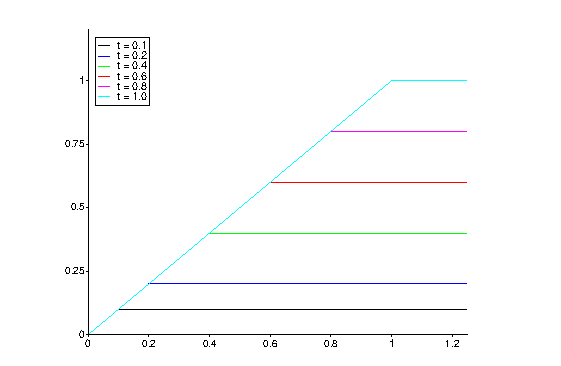
\includegraphics[width=0.9\textwidth]{cart_channel.pdf}
\end{center}
\end{figure}


\bibliography{boundary-initial}
\bibliographystyle{unsrt}
\end{document}
